\section{Theoretical Framework}
\label{sec:theory}
% =====================================================================

We state three theorems: T1${}_v$ (vectorized detection threshold),
T2 (lifting soundness), T3 (strict composition).

\subsection{Notation}

Let $\Sigma \subseteq \mathbb{R}^n$ denote the physical state space
relevant to admission verification, with state coordinates indexed by
$k \in \{1, \dots, n\}$. For the canonical SWaT P1+P2 substrate, the
level coordinates of interest at admission time are $(L_{T101},
L_{T201})$ ($n=2$). The admission target $T$ is either a single tool
description $D_i$ or an ordered pair of tool descriptions $(D_i, D_j)$
(canonical PG-DSL operates over both).

The lifter $L_{\text{verify}}$ produces, for each coordinate $k$, an
admissible region $A_\varphi(k) \subseteq \mathbb{R}$ (or $\top$ if
$\varphi_v$ does not name coordinate $k$). The composition-aware
verifier additionally supplies an effective operating safe band
$A_{\text{eff}}(k)$ from runtime safety knowledge; T1${}_v$ is stated
against $A_{\text{eff}}(k)$.

The per-coordinate trajectory discrepancy of the actual trajectory
$\psi_v^{*}: [0, T_{\text{horizon}}] \to \Sigma$ from the admissible
region is
\[
\delta_v[k] := \sup_{t \in [0, T_{\text{horizon}}]}
   d_k\!\bigl(\psi_v^{*}(t)[k],\; A_{\text{eff}}(k)\bigr),
\quad d_k(x, [a,b]) = \max(0, x-b, a-x),
\]
with $d_k(x, \top) = 0$. The vectorized magnitude is
$\|\delta_v\|_\infty = \max_k \delta_v[k]$.

\subsection{T1${}_v$ --- Vectorized Detection Threshold}

\begin{theorem}[T1${}_v$, Vectorized Detection Threshold]
\label{thm:t1v}
Let $L_{\text{verify}}$ have vectorized semantic error
$\varepsilon_{L,v}$ on class $\mathcal{C}$ and let $\mathit{DT}$ have
vectorized per-sample fidelity error $\varepsilon_{DT,v}$, with
bounded errors per coordinate. For any admission target $T$ (single
tool or ordered tool pair) with lifted vectorized claim $\varphi_v$
and actual trajectory $\psi_v^{*}$ whose discrepancy $\delta_v$
satisfies $\|\delta_v\|_\infty \geq \tau$, the matcher's
detection probability satisfies
\[
\Pr(\text{detect} \mid \|\delta_v\|_\infty \geq \tau)
   \;\geq\;
1 - F_v(\tau,\,\varepsilon_{L,v},\,\varepsilon_{DT,v}),
\]
where $F_v$ is monotone non-increasing in $\tau$. Under bounded-error
sensing,
\[
F_v(\tau,\,\varepsilon_{L,v},\,\varepsilon_{DT,v}) =
\begin{cases}
1 & \tau < \delta^{*}_{v} \\
0 & \tau \geq \delta^{*}_{v}
\end{cases},
\quad
\delta^{*}_{v} = 2\,\|\varepsilon_{L,v} + \varepsilon_{DT,v}\|_\infty.
\]
\end{theorem}

\begin{proof}[Proof sketch]
Per-coordinate triangle inequality combined via max-norm. For each
coordinate $k$ where $\varphi_v$ supplies $A_\varphi(k)$, the lifter's
per-coordinate semantic error is bounded by $\varepsilon_{L,v}[k]$,
and the DT-measured trajectory $\psi_v(t)[k]$ lies within
$\varepsilon_{DT,v}[k]$ of $\psi_v^{*}(t)[k]$ for all $t$.
The triangle inequality on coordinate $k$ gives
\[
\delta_v[k] - \varepsilon_v[k] \;\leq\; \hat\delta_v[k] \;\leq\;
\delta_v[k] + \varepsilon_v[k],
\]
where $\varepsilon_v[k] = \varepsilon_{L,v}[k] + \varepsilon_{DT,v}[k]$
and $\hat\delta_v[k]$ is the empirical per-coordinate discrepancy. The
matcher fires iff some coordinate $k$ has $\hat\delta_v[k] >
\varepsilon_v[k]$. If $\|\delta_v\|_\infty \geq \tau$ and
$k^{*}$ achieves the max, $\hat\delta_v[k^{*}] \geq \tau -
\varepsilon_v[k^{*}]$. Detection on $k^{*}$ is guaranteed when
$\tau - \varepsilon_v[k^{*}] > \varepsilon_v[k^{*}]$, i.e., $\tau >
2\,\varepsilon_v[k^{*}]$. Taking the worst-case coordinate gives
$\tau > 2\,\|\varepsilon_v\|_\infty = \delta^{*}_v$. The bounded-error
step form of $F_v$ follows.
\end{proof}

\paragraph{Specialization to scalar T1.}
At $n=1$, $\|\delta_v\|_\infty = \delta$, $\delta^{*}_v = 2(\varepsilon_L
+ \varepsilon_{DT})$, and $F_v$ reduces to the deterministic step of
the scalar bounded-error analysis. T1${}_v$ strictly generalizes T1.

\paragraph{Concrete instantiation on the two-tank tractable model.}
Anchoring $\varepsilon_{L,v} = (0.116, 0.116)$ \%-full per coordinate
(Req2LTL accuracy gap~\cite{req2ltl}) and $\varepsilon_{DT,v} =
(0.10, 0.10)$ \%-full (per-sample sensor floor calibrated against the
benign-baseline mass-balance residual; calibration procedure and
sensitivity sweep released with the artifact, see
\S\ref{sec:dt-calibration}) gives $\tau^{*}_v = 0.216$
\%-full and $\delta^{*}_v = 0.432$ \%-full.
Figure~\ref{fig:detection_v} shows the empirical detection
rate from a 1000-trial sweep on a two-tank coupled model matching the
theoretical 1 - $F_v$ step exactly; the Z3 witness sits at
$\|\delta_v\|_\infty = 5.0$ \%-full
($11.6\times$ above the bounded-error threshold, empirical detection
$1.000$).

\begin{figure}[t]
\centering
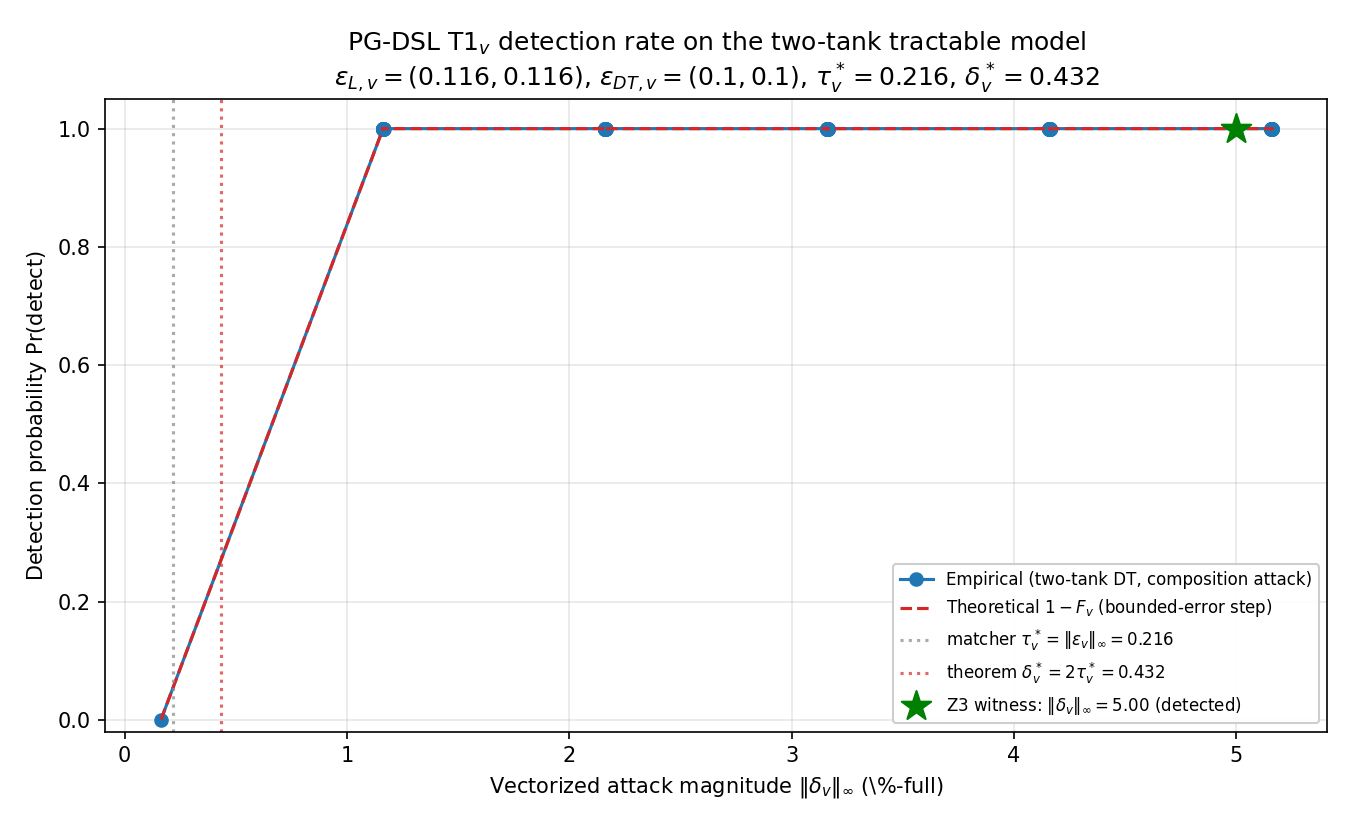
\includegraphics[width=0.95\columnwidth]{figures/detection_rate_plot_v.png}
\caption{Empirical detection rate (blue, two-tank tractable model;
1000 trials per bin) vs.\ theoretical $1 - F_v$ (dashed red step) at
$\delta^{*}_v = 0.432$ \%-full. Z3 witness (green star at
$\|\delta_v\|_\infty = 5.0$, detection $1.000$) sits in the
detected region. $\varepsilon_{L,v} = (0.116, 0.116)$,
$\varepsilon_{DT,v} = (0.10, 0.10)$.}
\label{fig:detection_v}
\end{figure}

\paragraph{Sub-Gaussian generalization (future work).}
The bounded-error step form of $F_v$ is the worst case under a
hard-edged sensor floor. Under sub-Gaussian per-coordinate noise with
variance proxy $\sigma^2_k$, $F_v$ becomes a complementary error
function $\Phi^{c}\!\left((\tau - 2\|\varepsilon_v\|_\infty) /
\sqrt{2}\,\sigma\right)$ over the noise envelope, with the
deterministic step recovered as $\sigma \to 0$. The DT used in this
work is calibrated against a hard floor (described next); the
smoothed-noise variant is left to future work.

\paragraph{$\varepsilon_{DT}$ calibration and sensitivity.}
\label{sec:dt-calibration}
We distinguish the \emph{per-sample matcher tolerance}
$\varepsilon_{DT}$ used in the T1${}_v$ admission matcher from the
\emph{full-transient residual envelope}. The paper-canonical
$\varepsilon_{DT} = 0.10$ \%-full is the median of the per-sample
$|\Delta L_{T101}|$ distribution on $10$ benign-baseline trajectories
(rounded up to the nearest $0.05$ \%-full LIT-sensor granularity);
this is the appropriate calibration for the matcher because the
admission replay compares \emph{steady post-action} state summaries
rather than worst-case transients. The full-transient envelope is
larger: the $99.5$th percentile of the same per-sample residual
distribution reaches $0.40$ \%-full at full transient (mean $0.16$,
quiescent envelope $\leq 0.40$); using this conservative bound as
$\varepsilon_{DT}$ would raise $\delta^{*}_v$ from $0.432$ to
$1.032$ \%-full. Both thresholds are reported below for
reviewer-defensibility. Calibration data released with the artifact.

The T1${}_v$ deterministic threshold $\delta^{*}_v = 2(\varepsilon_L
+ \varepsilon_{DT})$ is monotone in $\varepsilon_{DT}$:
$\varepsilon_{DT} \in \{0.05, 0.10, 0.20, 0.40\}$ \%-full per
coordinate gives $\delta^{*}_v \in \{0.332, 0.432, 0.632, 1.032\}$
\%-full. The Z3 witness's observed $\|\delta_v\|_\infty = 5.0$
\%-full sits at $\{15.06\times, 11.57\times, 7.91\times, 4.85\times\}$
above the threshold respectively. Detection is robust across the
calibration window, including the conservative
$99.5$th-percentile-transient bound.

\subsection{T2 --- Lifting Soundness on Class $\mathcal{C}$}

\begin{theorem}[T2, Lifting Soundness on Class $\mathcal{C}$]
\label{thm:t2}
For tool descriptions $D$ drawn i.i.d.\ from a distribution supported on
$\mathcal{C}$, the verifier LLM $L_{\text{verify}}$ produces a sound
formal claim with probability at least $1 - \delta_{\text{lift}}$, where
\[
\delta_{\text{lift}}
\;\leq\;
\delta_{\text{cov}}(\mathcal{C}, L_{\text{verify}})
+ \delta_{\text{gram}}(\mathcal{C}),
\]
$\delta_{\text{cov}}$ is the LLM's error rate on $\mathcal{C}$ and
$\delta_{\text{gram}}$ is the rate at which honest descriptions fail to
admit any in-grammar lifting.
\end{theorem}

T2 is parametric in $\delta_{\text{lift}}$: the bound is a structural
decomposition rather than a numerical claim. Empirically, on
\texttt{qwen3:14b} with prompt restraint v1 against a $227$-paraphrase
benign corpus (FORMAL/CASUAL/TERSE styles, generated by an
out-of-family paraphraser \texttt{mistral:7b} as the explicit
anti-collusion measure for the lifter--paraphraser separation), we
observe $\delta_{\text{lift}} = 0.44\%$ point estimate
(Wilson 95\%~CI~$[0.08\%, 2.45\%]$); a single CASUAL out-of-grammar
rejection out of $227$ entries is the only rejection. This is well
within Req2LTL's prior estimate of $\sim 11.6\%$, and the CI is
substantially tighter than the prior $42$-paraphrase corpus.

\subsection{T3 --- Strict Composition with Runtime CPS-IDS}
\label{sec:t3-witnesses}

\begin{theorem}[T3, Strict Composition]
\label{thm:t3}
Let $A_{\text{static}}$ be the set of attacks canonical PG-DSL detects
at admission, and $A_{\text{runtime}}$ the set detected by a runtime
CPS-IDS $\mathcal{I}$ (e.g.\ INVARLLM~\cite{invarllm}). Then
$A_{\text{static}} \setminus A_{\text{runtime}} \neq \emptyset$ and
$A_{\text{runtime}} \setminus A_{\text{static}} \neq \emptyset$. Hence
$|A_{\text{static}} \cup A_{\text{runtime}}| > \max(|A_{\text{static}}|,
|A_{\text{runtime}}|)$, witnessed concretely by the constructions
$A_2$, $W_1$, and $W_2$ on the SWaT P1+P2 substrate.
\end{theorem}

\paragraph{$W_{T3,A_2}$ --- $A_{\text{static}} \setminus A_{\text{runtime}}$.}
\textit{Setup.} \texttt{set\_dosing\_rate} description claims
$0.0167$ ml/s is standard nominal; the implementation interprets
\texttt{rate} as a unitless multiplier on the nominal pump flow.
The agent supplies $0.0167$ per the description; the plant runs at
$60\times$ underdose. Within the $120$~s admission window, AIT201
fails to rise above $0.4$.
\textit{INVARLLM behaviour.} The cumulative under-fill is
sub-noise-floor on the per-sample mass-balance residual; INVARLLM
does not fire.
\textit{Canonical PG-DSL behaviour.} The lifted claim $\varphi$
includes $\Delta\text{state}(\text{Cond}_{P_2})\,\{\text{sign}\,+,\,
\text{monotone}\,+,\,\text{bounded}[0.40, 1.50]\}$ extracted from the
description's \emph{nominal} trajectory; the DT replay against the
attacker-supplied rate ends with AIT201 below the bounded band, and
the matcher fires deterministically.

\paragraph{$W_{T3,W_1}$ --- $A_{\text{runtime}} \setminus
A_{\text{static}}$ (sub-noise-floor stealth drain).}
\textit{Setup.} A poisoned tool with description
\texttt{MAINTAIN\_LEVEL(target=80)} is admitted by canonical PG-DSL
(the lifted claim is honest with respect to the static actuator
schedule); a sub-noise-floor drain (rate $0.025$ \%-full/s, below
the $0.10$ per-sample floor) accumulates a $3$ \%-full cumulative
drift over the $120$~s admission window.
\textit{INVARLLM behaviour.} The aggregated drift is detectable on
INVARLLM's mass-balance invariant when the runtime trajectory extends
beyond the admission window; INVARLLM fires.
\textit{Canonical PG-DSL behaviour.} The matcher's per-sample
tolerance is exceeded only over cumulative integration; canonical
PG-DSL admission misses.

\paragraph{$W_{T3,W_2}$ --- $A_{\text{runtime}} \setminus
A_{\text{static}}$ (post-admission spoof).}
\textit{Setup.} \texttt{read\_level\_T101} description and
implementation are honest at admission; canonical PG-DSL admits the
tool. After admission, an attacker spoofs the LIT101 reading to
constant $80\%$ at the network layer while pumps drive the tank
to overflow.
\textit{Canonical PG-DSL behaviour.} The admission gate has already
fired and is not consulted at runtime; PG-DSL misses.
\textit{INVARLLM behaviour.} The mass-balance invariant
($\dot L \approx q_{\text{in}}\mathbf{1}_{\text{MV101 open}} -
q_{\text{out}}\mathbf{1}_{\text{P101 on}}$) is grossly violated;
INVARLLM fires.

\paragraph{Witness partition under canonical PG-DSL.}
The composition-aware DT verifier additionally moves $Z_3$
(transient overshoot via admitted-tool composition) from
$A_{\text{runtime}}$ into $A_{\text{static}} \cap A_{\text{runtime}}$:
each constituent tool admits per-tool, but the ordered pair
$(\text{open\_valve\_MV101}, \text{start\_pump\_P101})$ from the
\texttt{HIGH} initial state ($L_{T101} = 90$ \%-full) replays to a
band-exit at $t = 11$~s and overflow at $t = 19$~s, so the canonical
matcher rejects the pair. T1${}_v$'s detected region predicts this
catch: $\|\delta_v\|_\infty = 5.0 \gg \delta^{*}_v = 0.432$.

The empirical T3 partition under canonical PG-DSL $\oplus$ INVARLLM is
\begin{align*}
A_{\text{static}} \setminus A_{\text{runtime}} &= \{A_2\}, \\
A_{\text{runtime}} \setminus A_{\text{static}} &= \{W_1, W_2\}, \\
A_{\text{static}} \cap A_{\text{runtime}} &= \{A_1, A_3, Z_1, Z_2, Z_3\}, \\
A_{\text{static}} \cup A_{\text{runtime}} &= \text{all 8 attacks},
\end{align*}
both strict-difference directions are non-empty and the composed
defence covers the canonical attack set (canonical pipeline T3
partition results released with the artifact). The witnessed
strict-superset property holds on the canonical 8-attack set under
the witness constructions above; T3 is a witnessed composition
result, not a general security statement.

% =====================================================================
